\chapter{PCB Design}
\label{cap:pcbdesign}

Following the initial development on a breadboard, the natural progression in the design evolution was to 
transition to a perfboard assembly. This intermediate step not only served to condense the device's 
footprint but also offered a preliminary glimpse into its form and functionality. Subsequently, the 
culmination of this iterative process involved the design and fabrication of a PCB tailored to the 
project's specifications, marking a significant milestone in its realization.


\section{Assembling on a Perfboard}

Perfboards, short for perforated boards, are commonly used prototyping platforms in electronics. They 
consist of a board with a grid of holes spaced at regular intervals. These holes are surrounded by copper 
pads or traces that can be connected using solder to create electronic circuits. Perfboards allow 
electronic components, such as resistors, capacitors, integrated circuits, and other discrete components, 
to be soldered onto the board, facilitating the creation of temporary or semi-permanent circuits for 
testing and development purposes \cite{perfboard}. They serve as a practical and versatile tool for 
electronics hobbyists, engineers, and designers to quickly prototype and iterate on circuit designs 
before moving to more permanent solutions like printed circuit boards (PCBs). Examples can be seen in 
Figures \ref{fig:perfboard_back} and \ref{fig:perfboard_front}.

\begin{figure}[h]
    \centering
    \begin{minipage}[b]{0.45\textwidth}
        \centering
        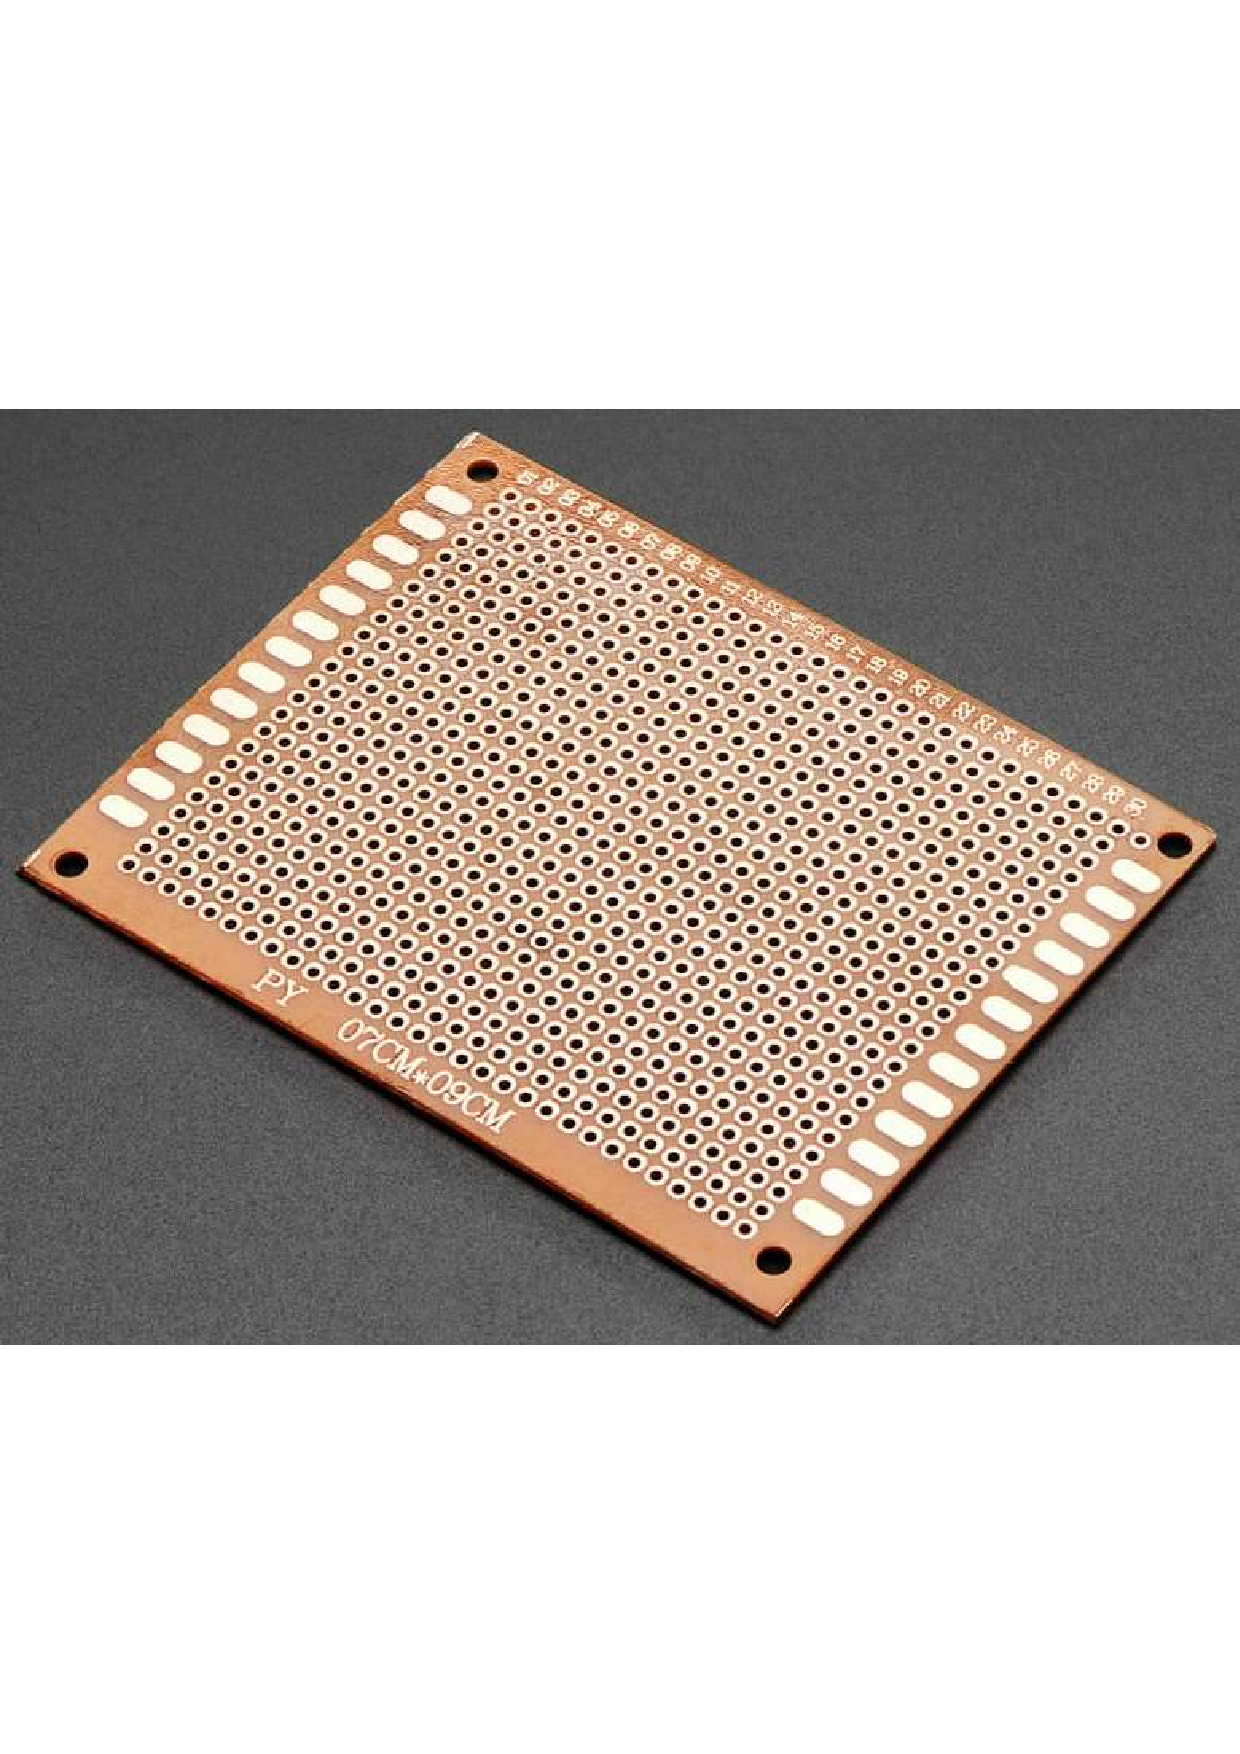
\includegraphics[width=.8\textwidth]{Imagenes/Vectorial/perfboard_back.pdf}
        \caption{Back side of a perfboard}
        \label{fig:perfboard_back}
    \end{minipage}
    \hfill
    \begin{minipage}[b]{0.45\textwidth}
        \centering
        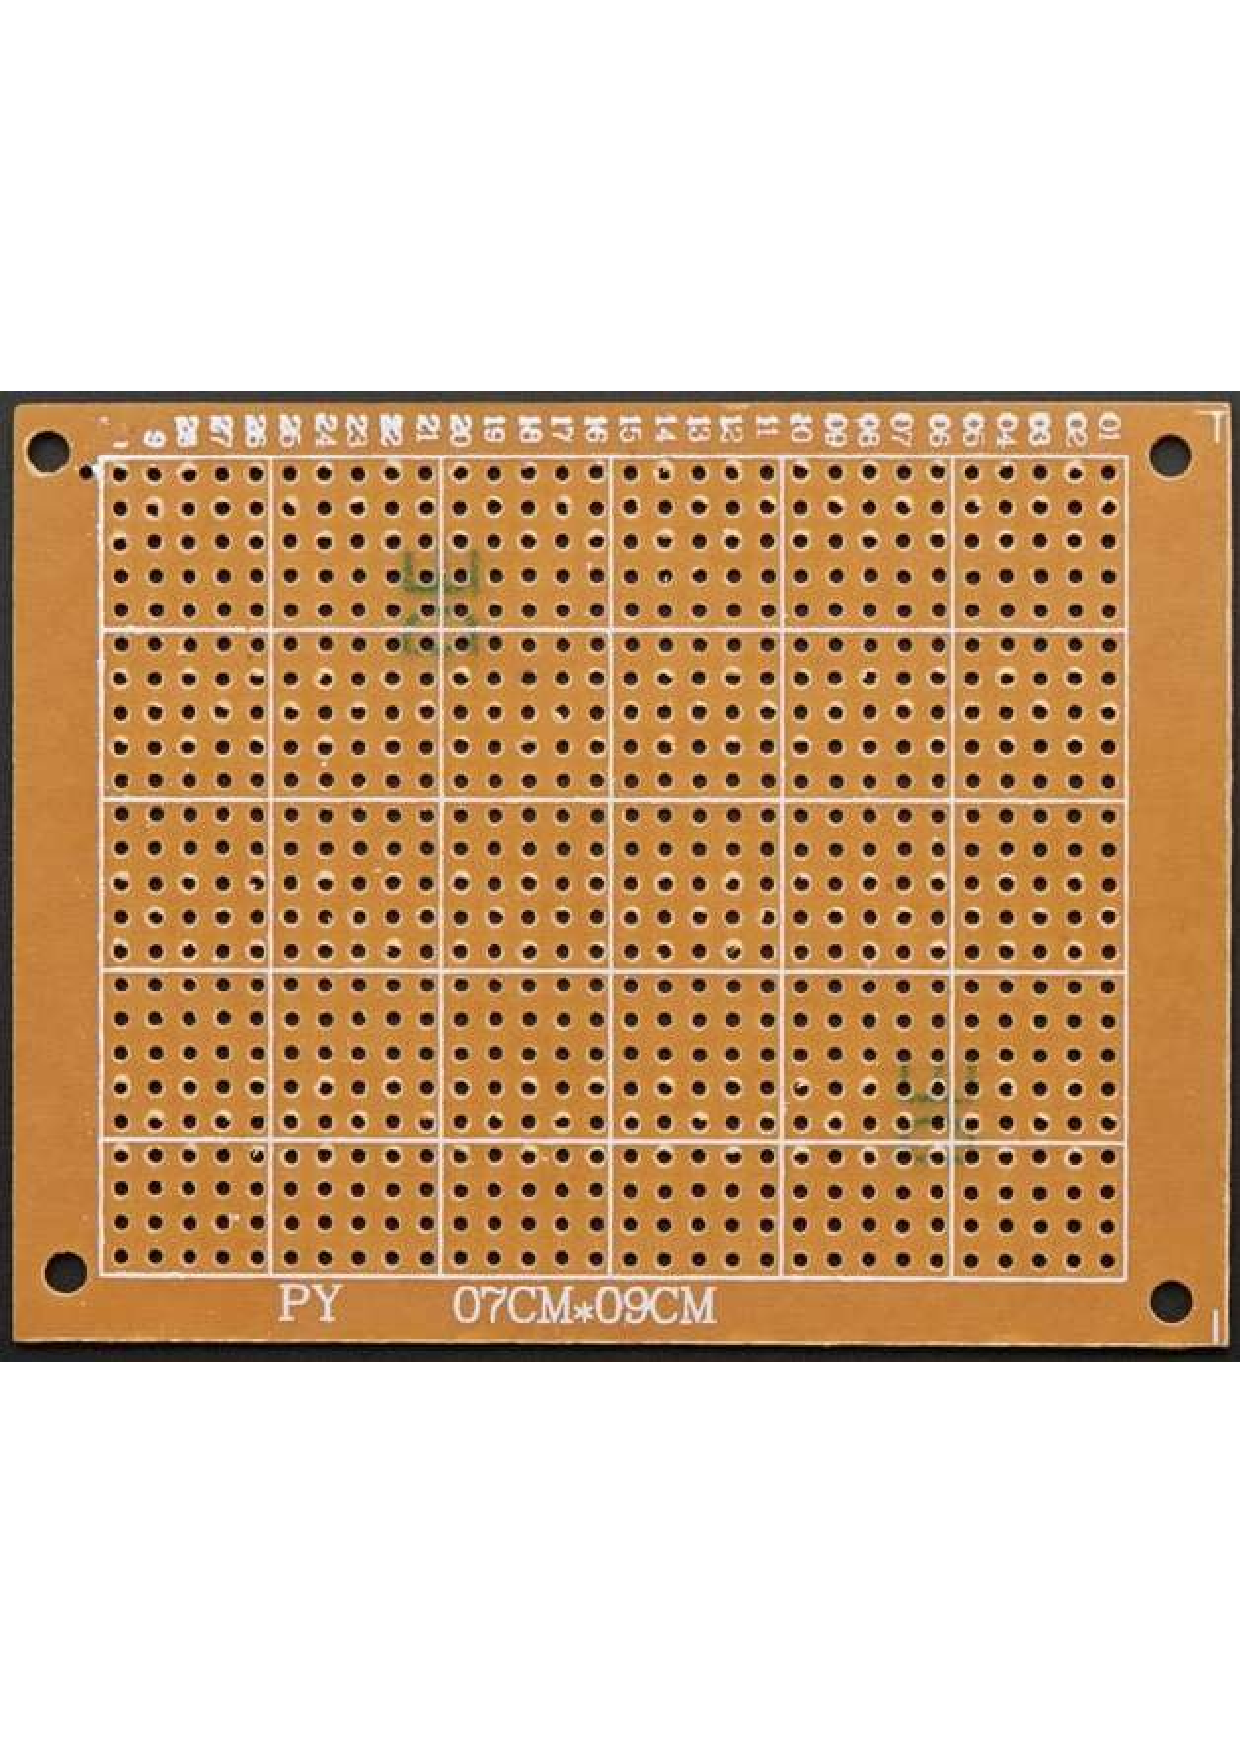
\includegraphics[width=.8\textwidth]{Imagenes/Vectorial/perfboard_front.pdf}
        \caption{Front side of a perfboard}
        \label{fig:perfboard_front}
    \end{minipage}
\end{figure}

In the context of this project, transitioning to a perfboard prototype served multiple crucial purposes. 
Firstly, it offered a tangible visualization of the future device's physical footprint, providing 
executives with a concrete representation of the project's direction and potential. This visual aid not 
only conveyed the scale and form of the device but also showed its feasibility and progress, instilling 
confidence in its development trajectory.

To commence this phase, a diagram detailing the placement of each component and its connection to the 
corresponding pins on the microcontroller was drafted. This diagram served as a blueprint, guiding the 
subsequent assembly process.

With the schematic as a roadmap, the assembly of the perfboard prototype commenced. Components were 
transitioned from the breadboard to the perfboard, ensuring each element found its designated place. 
Careful consideration was given to the layout, optimizing spatial organization for efficient circuitry 
and minimal interference.

\begin{figure}[h]
    \centering
    \begin{minipage}[b]{0.45\textwidth}
        \centering
        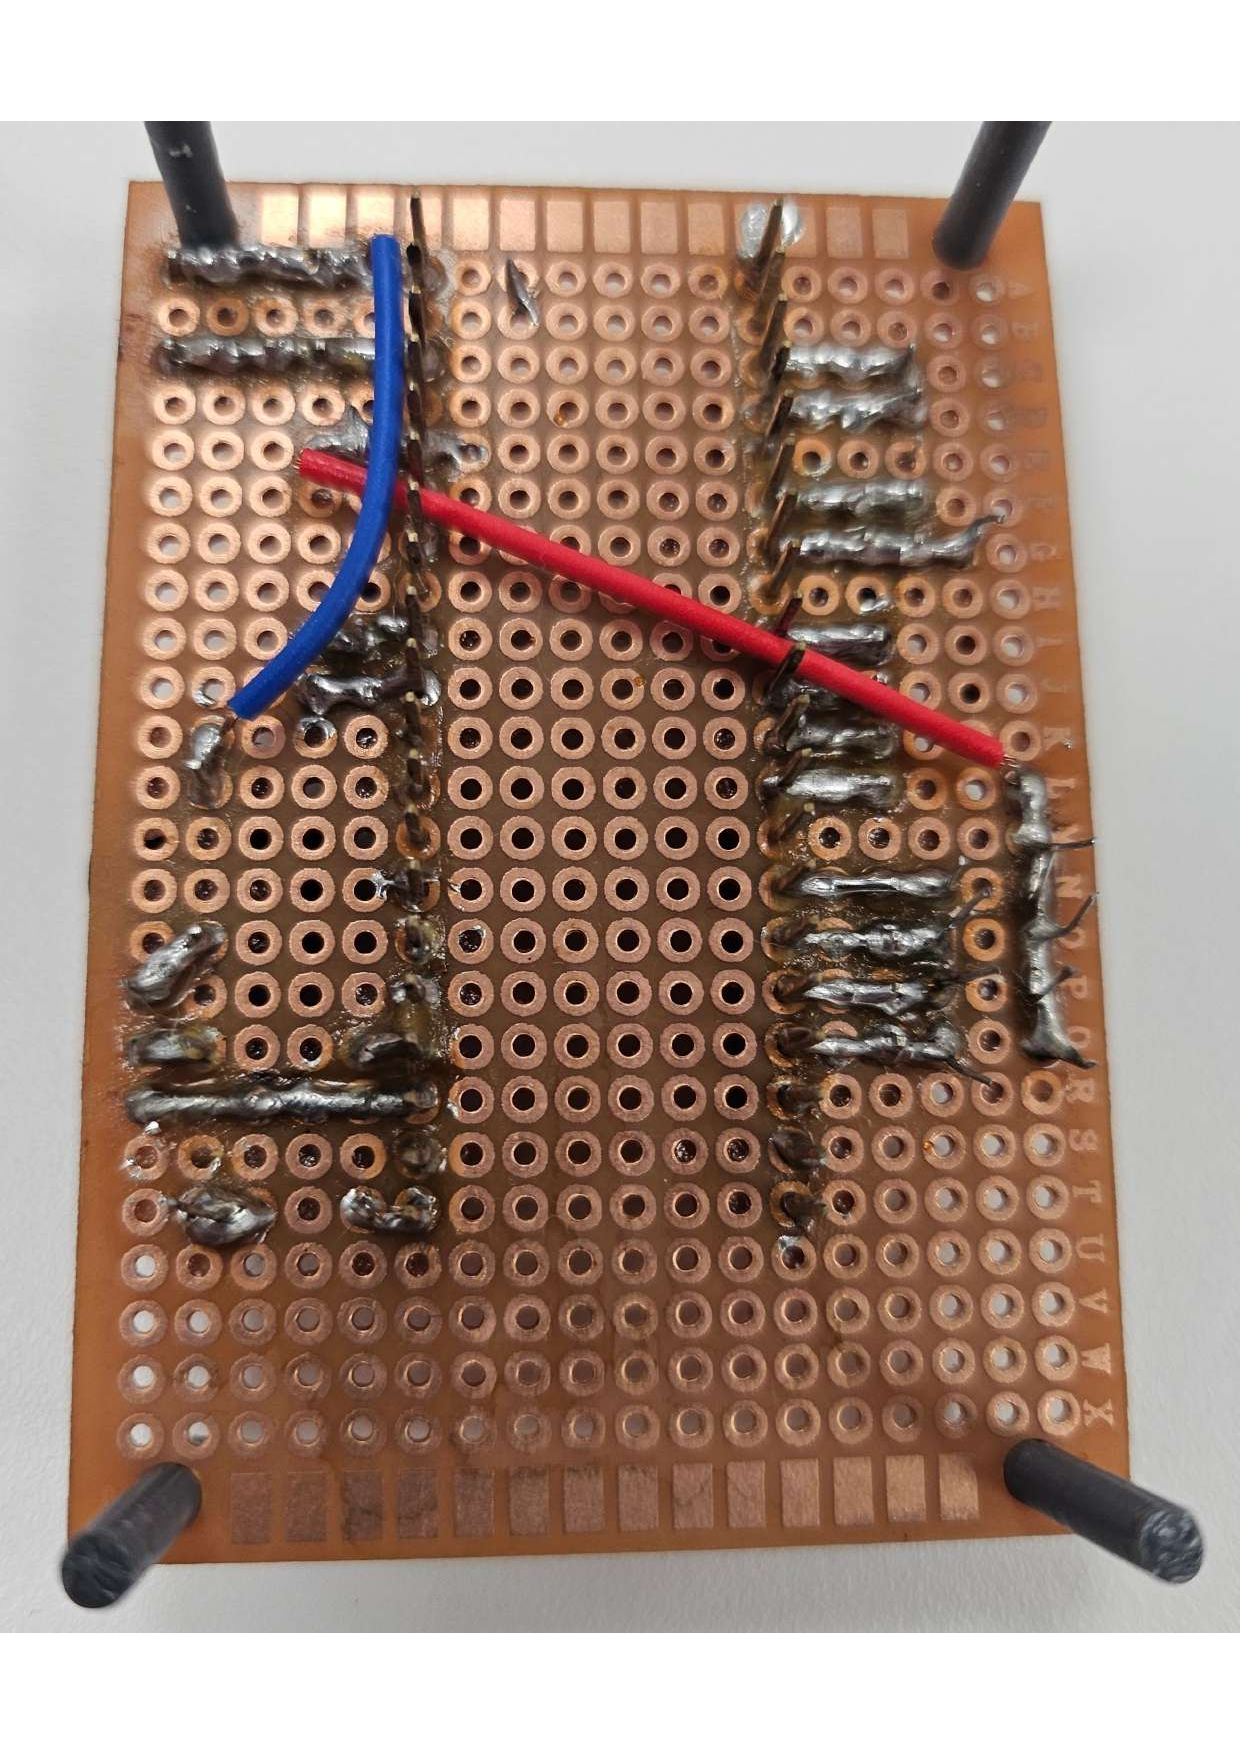
\includegraphics[width=.8\textwidth]{Imagenes/Vectorial/perfboard_assembled_back.pdf}
        \caption{Back side of the assembled perfboard}
        \label{fig:perfboard_assembled_back}
    \end{minipage}
    \hfill
    \begin{minipage}[b]{0.45\textwidth}
        \centering
        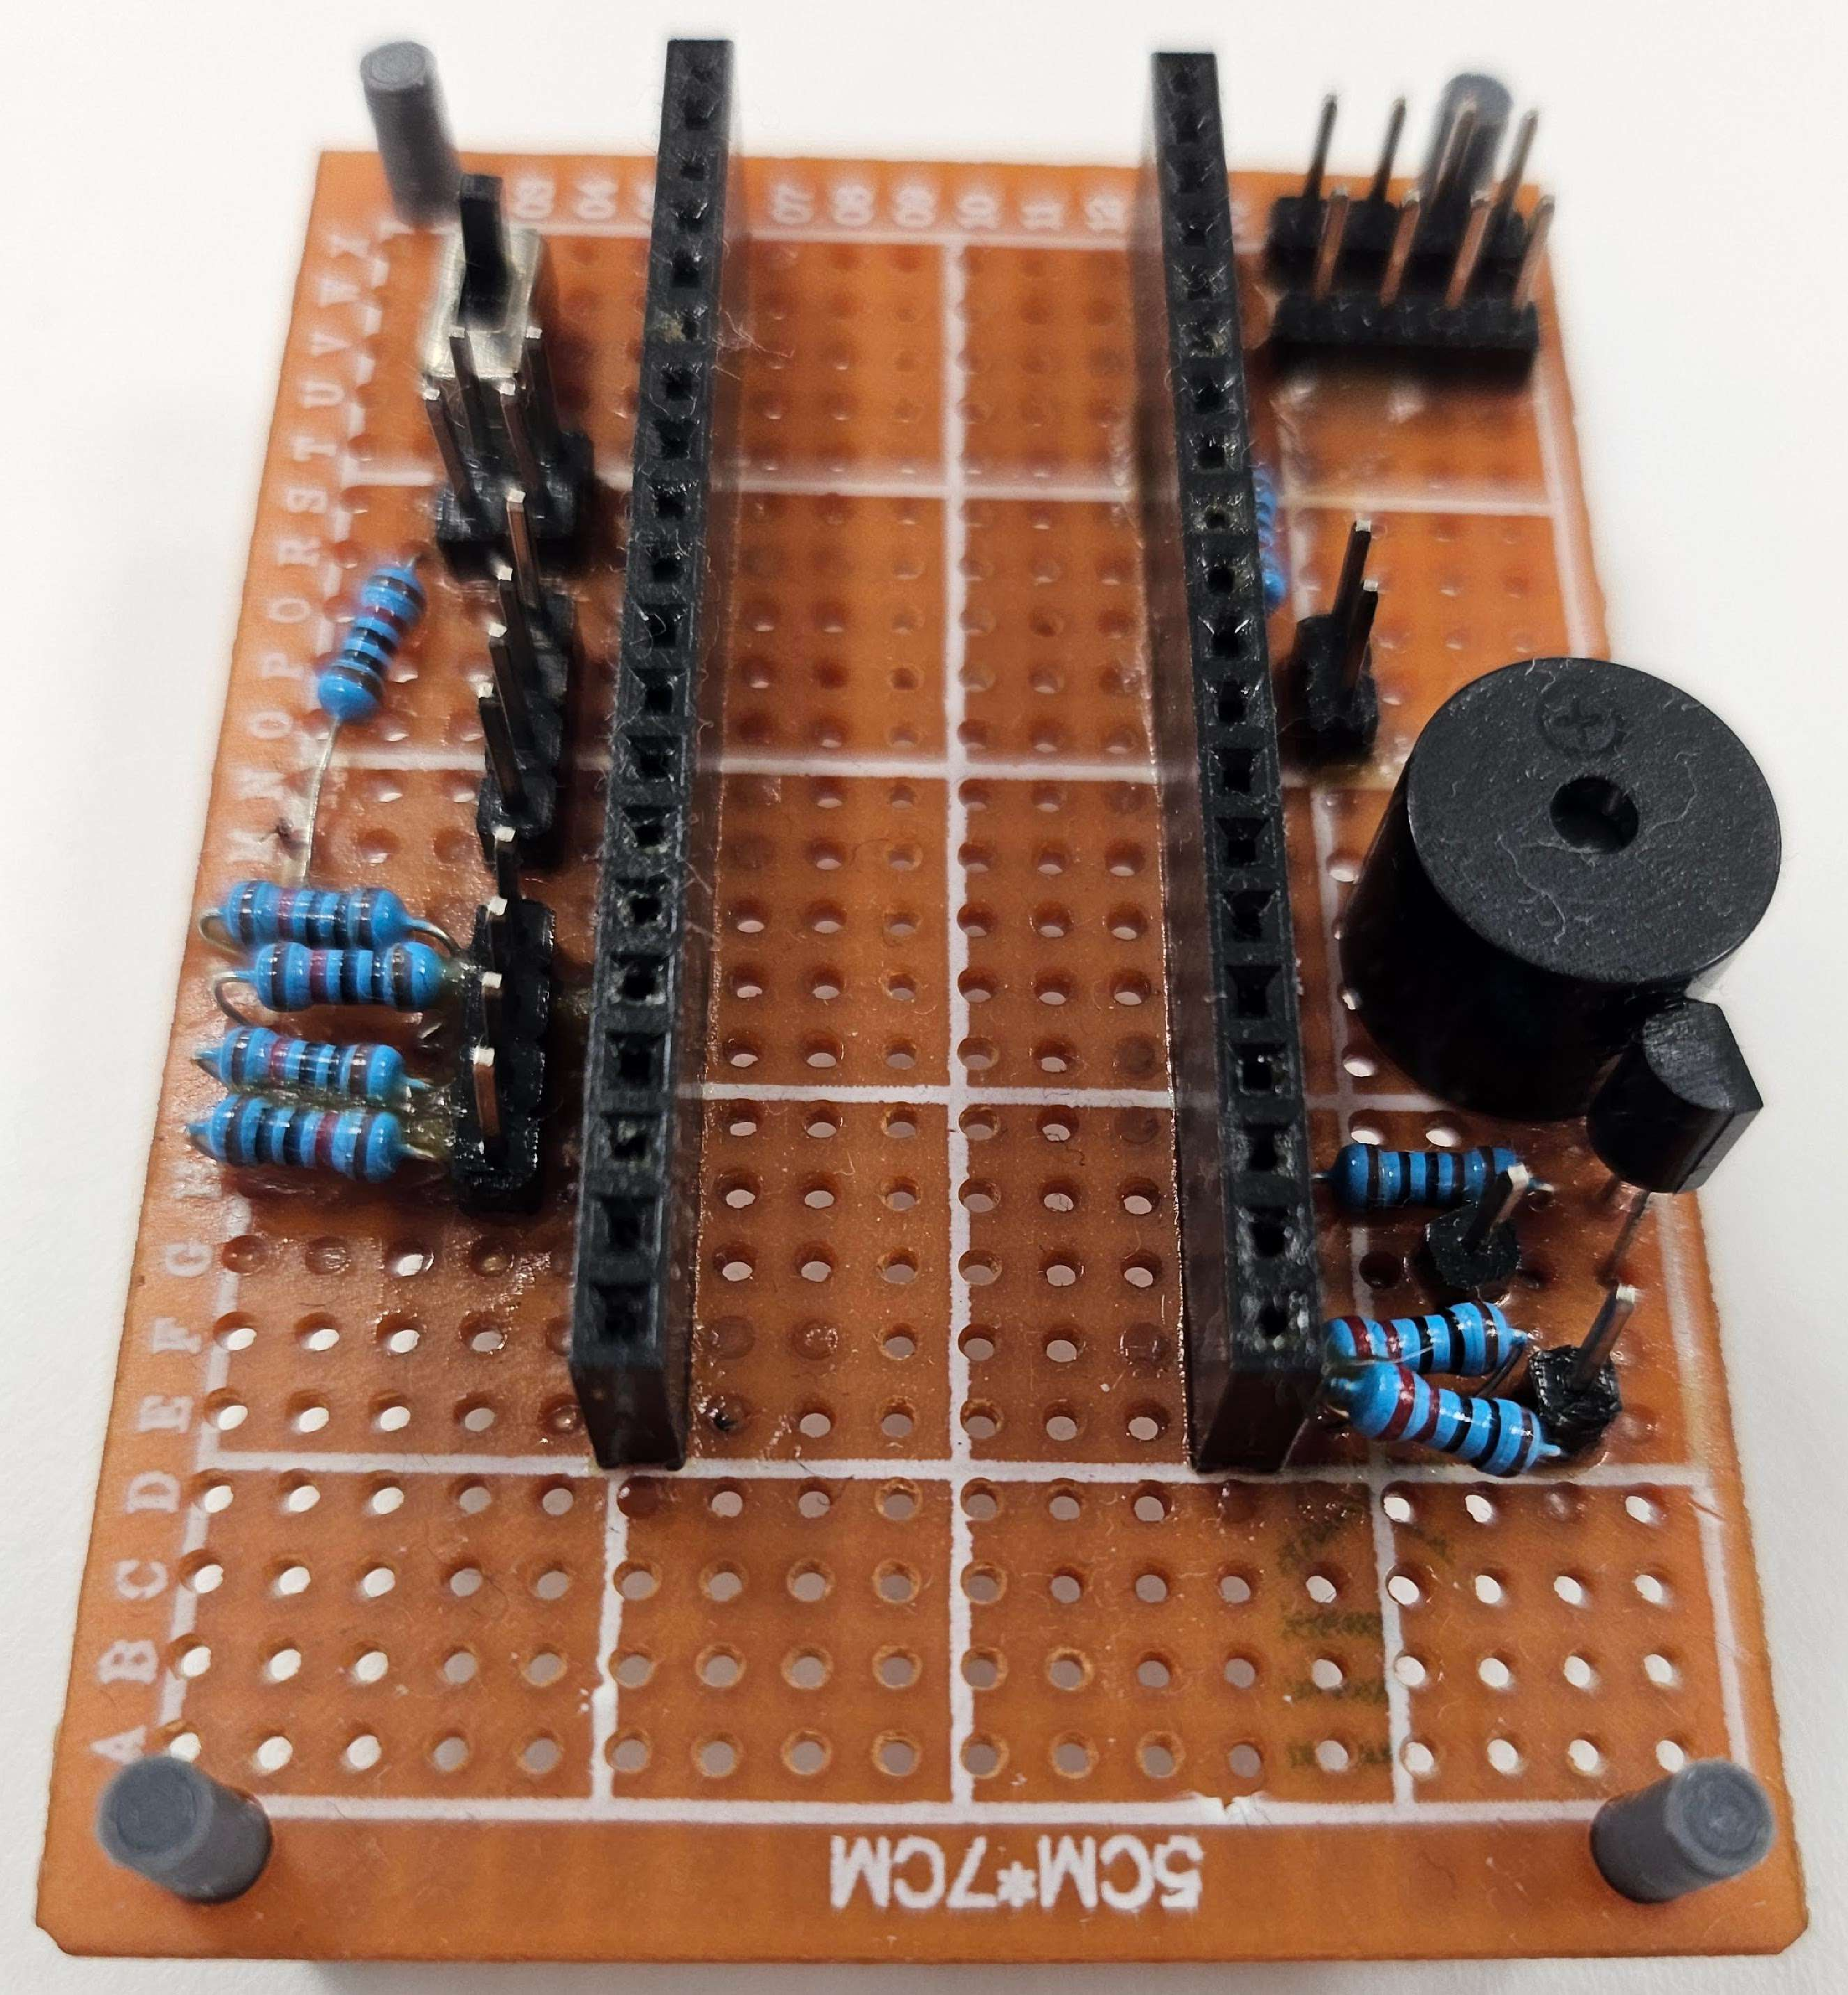
\includegraphics[width=.8\textwidth]{Imagenes/Vectorial/perfboard_assembled_front.pdf}
        \caption{Front side of the assembled perfboard}
        \label{fig:perfboard_assembled_front}
    \end{minipage}
\end{figure}


\section{Designing the PCB}

Now that the perfboard provided a good idea of how the PCB could be, now it has to be properly designed. As it could be seen before, the perfboard's main job was to bring all components together, and that will also be the case for the PCB. It would give a much cleaner look than the perfboard, and be much more comfortable to plug components into, since on the perfboard traces could not overlap, limiting design possibilities. Now, with a multi-layer PCB, traces could go above and below each other, allowing for the placement continuous male headers for each component.

Having used the perfboard as a preliminary platform to consolidate components and understand the spatial dynamics of the circuit, the focus now shifts towards the meticulous design of the printed circuit board (PCB).

The primary function of the PCB mirrors that of the perfboard: to integrate and interconnect all components seamlessly. However, unlike the perfboard, the PCB offers advantages in terms of aesthetics, functionality, and ease of assembly.

Moreover, the transition to a multi-layer PCB introduces a realm of design possibilities previously unattainable with the perfboard. By using multiple layers, traces can now traverse both above and below the surface, allowing for more flexibility in component placement and routing. This feature allows for the implementation of continuous male headers for each component, which were not easily implemented with the perfboard.
